The differential cross-section measurements discussed in this thesis are affected by three sources of systematic uncertainties, experimental sources, theoretical sources, and intrinsic systematics related to the unfolding process. The statistical uncertainty of the measurements is dominant as data statistics limit the cross-section measurements. This section discusses the source of theoretical, experimental, unfolding uncertainties and propagation of the statistical uncertainties to the unfolded cross-sections. 

\subsection{Theoretical Uncertainties}
\label{subsec:TheoryUnc}

The following sources of theoretical uncertainties are considered in the measurement.

\begin{itemize}
\item{\textbf{Uncertainties on QCD Scale:} As discussed in Section \ref{sec:Pheno}, the theoretical predictions of cross-sections depend on the factorization scale ($\mu_{F}$) and renormalization scale ($\mu_{R}$) \cite{QCDScaleAndPDFUnc}. To account for this dependence, a QCD scale uncertainty is evaluated by scaling $\mu_{F}$ and $\mu_{R}$ independently using on-the-fly variations provided by the MC generators. The variations constitute of six-point variations of $\mu_{F}$ and $\mu_{R}$ from $-50\%$ or $+100\%$ around their nominal values of 1, such that \{$\mu_R = 0.5, \mu_F = 0.5$\}, \{$\mu_R = 0.5, \mu_F = 1.0$\}, \{$\mu_R = 1.0, \mu_F = 0.5$\}, \{$\mu_R = 1.0, \mu_F = 2.0$\}, \{$\mu_R = 2.0, \mu_F = 1.0$\}, and \{$\mu_R = 2.0, \mu_F = 2.0$\}. The final uncertainty is evaluated as the absolute envelope of the six variations. The QCD scale uncertainties are evaluated for $qqZZ$, $ggZZ$, and $EWK qqZZjj$ samples. \textcolor{red}{to add intermediate systematics plot} %Figure \ref{fig:QCDScale} shows different variations and the final envelope for QCD Scale uncertainties in the VBS Enhanced region as a function of $m_{jj}$. 

% \begin{figure}
%     \centering
%     \includegraphics[width=.8\linewidth]{figures/AnalysisOverview/mu_ProfileRun2.pdf}
%     \caption{ Evaluation of the fiducial level QCD factorization and renormalization scale uncertainties band for $qqZZ$ sample. \label{fig:QCDScale}}
% \end{figure}
}
\item{\textbf{Uncertainties on PDF $\&$ $\alpha_{S}$:} The cross-sections also depend on the choice of the PDF used by the MC generators. Thus, the PDF uncertainty for Sherpa and \textsc{MadGraph5} samples that use NNPDF3.0NNLO is evaluated using the prescription described in Ref \cite{PDFForRunII} using on-the-fly variation weights. The PDF variations include a set of 100 internal variations, two additional variations from the nominal PDF reweighted to the alternative MMHT2014nnlo \cite{MMHT2014PDFs} $\&$ CT14nnlo \cite{CT14nnlo} PDF sets and variations of the strong coupling constant by $\pm0.0001$ where the nominal value of $\alpha_{S}$ is $0.118$. The total uncertainty is taken as the absolute envelope of all standard deviations of $100$ internal variations, the two alternate PDF variations, added in quadrature with the envelope of the $\alpha_{S}$ variations, 
\begin{equation}
    \sigma_{PDF}^{NNPDF3.0NNLO} = \sqrt{ [ max (\sigma_{std.~dev.~int.}, |\sigma_{MMHT2014nnlo}| , |\sigma_{CT14nnlo}|~)]^2 + \sigma_{\alpha_S}^2 }
\end{equation}

The PDF uncertainty is evaluated for $qqZZ$, $ggZZ$ and \textsc{MadGraph5} $EWK qqZZjj$ samples. \textcolor{red}{to add intermediate systematics plot}  %Figure \ref{fig:PDFScale} shows different variations and the final envelope for QCD Scale uncertainties in the VBS Enhanced region as a function of $m_{jj}$. 

% \begin{figure}
%     \centering
%     \includegraphics[width=.8\linewidth]{figures/AnalysisOverview/mu_ProfileRun2.pdf}
%     \caption{ Evaluation of the fiducial level QCD factorization and renormalization scale uncertainties band for $qqZZ$ sample. \label{fig:PDFScale}}
% \end{figure}

The electroweak $EWK~qqZZjj$ samples generated by \textsc{POWHEG-V2} do not have on-the-fly variations to evaluate the PDF uncertainty. Therefore, PDF uncertainty from the \textsc{MadGraph5} sample is taken as the PDF uncertainty for \textsc{POWHEG-V2} $EWK~qqZZjj$ samples.
}

\item{\textbf{Uncertainties on $gg\rightarrow ZZ^{(\ast)}$ NLO Corrections:}
The uncertainty is related to the NLO QCD k-factor applied to the $ggZZ$ sample \cite{ggZZNLOUnc}. The NLO QCD k-factors applied are evaluated differentially as a function of the $m_{4\ell}$. 
}

\item{\textbf{$t\bar{t}V$ $\&$ $VVV$ cross-sections:}
The experimental uncertainties on recently published cross-section measurements of the $ttV$~\cite{ATLAS_ttV} and $WZZ$~\cite{ATLAS_VVV} processes by ATLAS are propagated for the analysis. On the entire $ttV$ process, a flat conservative variation of $15\%$ is applied, taken from the cross-section measurement of $ttZ$. Similarly, for $VVV$ conservative $10\%$ variation taken from the cross-section measurement of $WWZ$ is applied to the whole $VVV$ samples.
}

\end{itemize}

As shown above, the theoretical uncertainties are process specific and are evaluated separately for each MC sample. The theory uncertainties need to be propagated to the unfolded cross-section measurements. For each theory uncertainty, variation-applied particle and detector level yields are built by substituting the varied distribution for the selected process instead of the nominal one. The variation-applied detector level yield is unfolded using the unfolding inputs from nominal SM predictions. The difference between the unfolded result to the variation-applied truth MC yields gives systematic uncertainty for each variation. In general, the theoretical variations significantly affect the predicted particle-level and detector-level yields; however, they have a negligible impact on the shape of the distributions. Since the variation is applied to both detector and particle level yields, the resulting uncertainties from theory systematics on the unfolded cross-sections are small.

\subsection{Experimental Uncertainties}
\label{subsec:ExpUnc}
The experimental uncertainties arise from the measurement of the energy and momentum scales of the reconstructed objects and the uncertainties on object reconstruction, identification, and selection efficiencies. The following category summarizes the sources of experimental uncertainties,

\textbf{Jet Related Uncertainties: }
The analysis requires two jets in the final state. Therefore, jet reconstruction and selection uncertainties are the measurement's most significant source of systematic experimental uncertainties. 

\begin{itemize}
    \item{\textbf{Jet Reconstruction Uncertainty:}
    The jet-related uncertainties associated with reconstruction and different steps of calibration discussed in Section \ref{subsec:ParticleRecon_Jets} are provided by ATLAS-supported tool $\textit{JetUncertainties}\footnote{https://twiki.cern.ch/twiki/bin/view/AtlasProtected/JetUncertainties}$. The tool provides several configurations for jet-related uncertainties adjusted to the various needs of several analyses. The measurement in this thesis uses $\textit{GlobalReduction\_FullJER}$ configuration with a total of $36$ uncertainties, each with upward and downward components, corresponding to $36\times2$ variations, $20\times 2$ variations are related to JES, and $13\times2$ to JER. $6\times 2$ of the $36 \times 2$ variations are related to the $\eta$ inter-calibration procedure, $4\times 2$ to the pile-up energy subtraction procedure, and $8 \times 2$ to the in-situ calibration of jets. Additional $1\times 2$ variations arise separately from the flavor composition, flavor response, a single particle response at high $p_{T}$, and possible punch-through effects.
    }
    \item{\textbf{JVT $\&$ fJVT Uncertainties:} Additional sets of jet uncertainties ($1\times 2$) arising from the efficiencies of jet vertex selections, JVT, and fJVT cut requirements are also considered in the analysis. }
\end{itemize}

An envelope of the $13$ JER uncertainty added in quadrature to an envelope of each of the other sources gives the final impact of jet-related uncertainties. 

\textbf{Lepton Related Uncertainties: } The following categories define the lepton-related uncertainties in the analysis
\begin{itemize}
    \item{\textbf{Electron Efficiencies:}
    The electron efficiency uncertainty consists of uncertainties on the trigger, identification, reconstruction,
and isolation efficiencies of electrons. These uncertainties are provided by an ATLAS-supported
tool $\textit{ElectronEffciencyCorrection} \footnote{https://gitlab.cern.ch/atlas/athena/-/tree/21.2/PhysicsAnalysis/ElectronPhotonID/ElectronEfficiencyCorrection} $. There are a total of $61$ nuisance parameters related to electron efficiencies, each with upward and downward components corresponding to $61\times2$ variations. $34\times2$ out of $61$ is related to uncertainties in identification efficiency, $25\times2$ related to the reconstruction efficiencies, and a single nuisance parameter ($1\times2$) each from the isolation efficiency and trigger efficiency scale factors.    
    }
    \item{\textbf{Muon Efficiencies:} Similar to the electrons, muon efficiency uncertainty consists of variations on the trigger, identification, reconstruction, and isolation efficiencies of muons, which are provided by another ATLAS-supported tool $\textit{MuonEfficiencyCorrections} \footnote{21https://gitlab.cern.ch/atlas/athena/-/tree/21.2/PhysicsAnalysis/MuonID/MuonIDAnalysis/MuonEfficiencyCorrections} $. In total, there are $10\times2$ nuisance parameters, sets of two ($2\times2$) variations corresponding to trigger efficiency scale factors, sets of four ($4\times2$) related to the identification and reconstructed efficiency, two sets of two ($2\times 2$) each corresponding to the isolation efficiency and track-to-vertex association efficiency. 
    }
    \item{\textbf{Electron Scale $\&$ Resolution:} The electron scale and resolution uncertainty is accounted for by two sets of nuisance parameters corresponding $2\times2$ variations. 

    }
    \item{\textbf{Muon Scale $\&$ Resolution:} For muons resolution and scale uncertainties, there are $5$ sets of nuisance parameters, $2\times2$ corresponding to the muon momentum resolution as measured separately by the Inner Detector and the Muon Spectrometer. One set of nuisance parameters ($1\times 2$) corresponds to the uncertainties on the muon momentum scale, and two sets of $2\times 2$ are associated with the uncertainties in Sagitta correction.}
\end{itemize}

\textbf{Other Experimental Uncertainties: }
\begin{itemize}
    \item{\textbf{Pileup Reweighting:} As discussed in Section \ref{subsec:EventWt}, the MC predictions are reweighted to match the pile-up profile of data. A single $1\times2$ nuisance parameter accounts for upward and downward variations in the factors used for pile-up reweighting. }
    \item{\textbf{Luminosity:} As discussed in Section \ref{subsec:Dataset}, the uncertainty in the collected integrated luminosity of $139 fb^{-1}$ is $\pm1.7\%$, which is applied as a flat variation to both particle and detector level yields. } 
\end{itemize}

The experimental uncertainties affect all detector-level MC predictions and the estimate of the fake backgrounds. The experimental uncertainties need to be propagated to the unfolded cross-sections. For each systematic variation, a detector-level signal ($qqZZ+ggZZ+EWK~qqZZjj$) and background ($ttV+VVV$) distribution, a variation applied prediction is built. The variation is also applied to the fake background estimate. The variation-applied background MC and fake backgrounds are subtracted from the variation-applied total MC prediction and then unfolded using the unfolding inputs from the nominal SM prediction. The individual systematic uncertainty corresponds to the difference between the variation-applied and nominal unfolded distributions for each variation.  

\subsection{Unfolding Uncertainties}
\label{subsec:UnfoldingUnc}
The following two uncertainties are intrinsic to the unfolding process itself and are included in the uncertainties for the unfolded differential cross-sections.

\begin{itemize}
    \item{\textbf{Unfolding Bias:} The unfolding bias estimated using the data-driven method discussed in Section \ref{subsec:Bias} is an inherent bias of the unfolding method and the biggest source of the systematic uncertainty for the measurement.
    }

    \item{\textbf{QCD $qqZZ$ Modeling Uncertainty:} There are known differences between different generators driven by differences in parton shower and hadronization. Therefore, the second source of unfolding systematics is required to account for the differences in the unfolding input modeling for the dominant $qqZZ$ process. To avoid double-counting of the unfolding method covered by the data-driven uncertainties, an alternative $qqZZ$ sample predicted by \textsc{MadGraph5} is first reweighted to match the nominal-\textsc{Sherpa} lineshape. The relative difference in reweighted detector-level distribution is unfolded using the inputs from nominal-\textsc{Sherpa} and compared with the reweighted-\textsc{MadGraph5} particle level distribution. The relative difference between these two distributions is taken as modeling systematic uncertainty. Figure \ref{fig:QCDModelUnc} shows the estimation of the modeling uncertainty for $m_{jj}$ in the VBS-Enhanced region. The ratio panel of the right plot shows the QCD modeling uncertainties, which range from $2-4\%$ varying in different bins.
    
    \begin{figure}
        \centering
        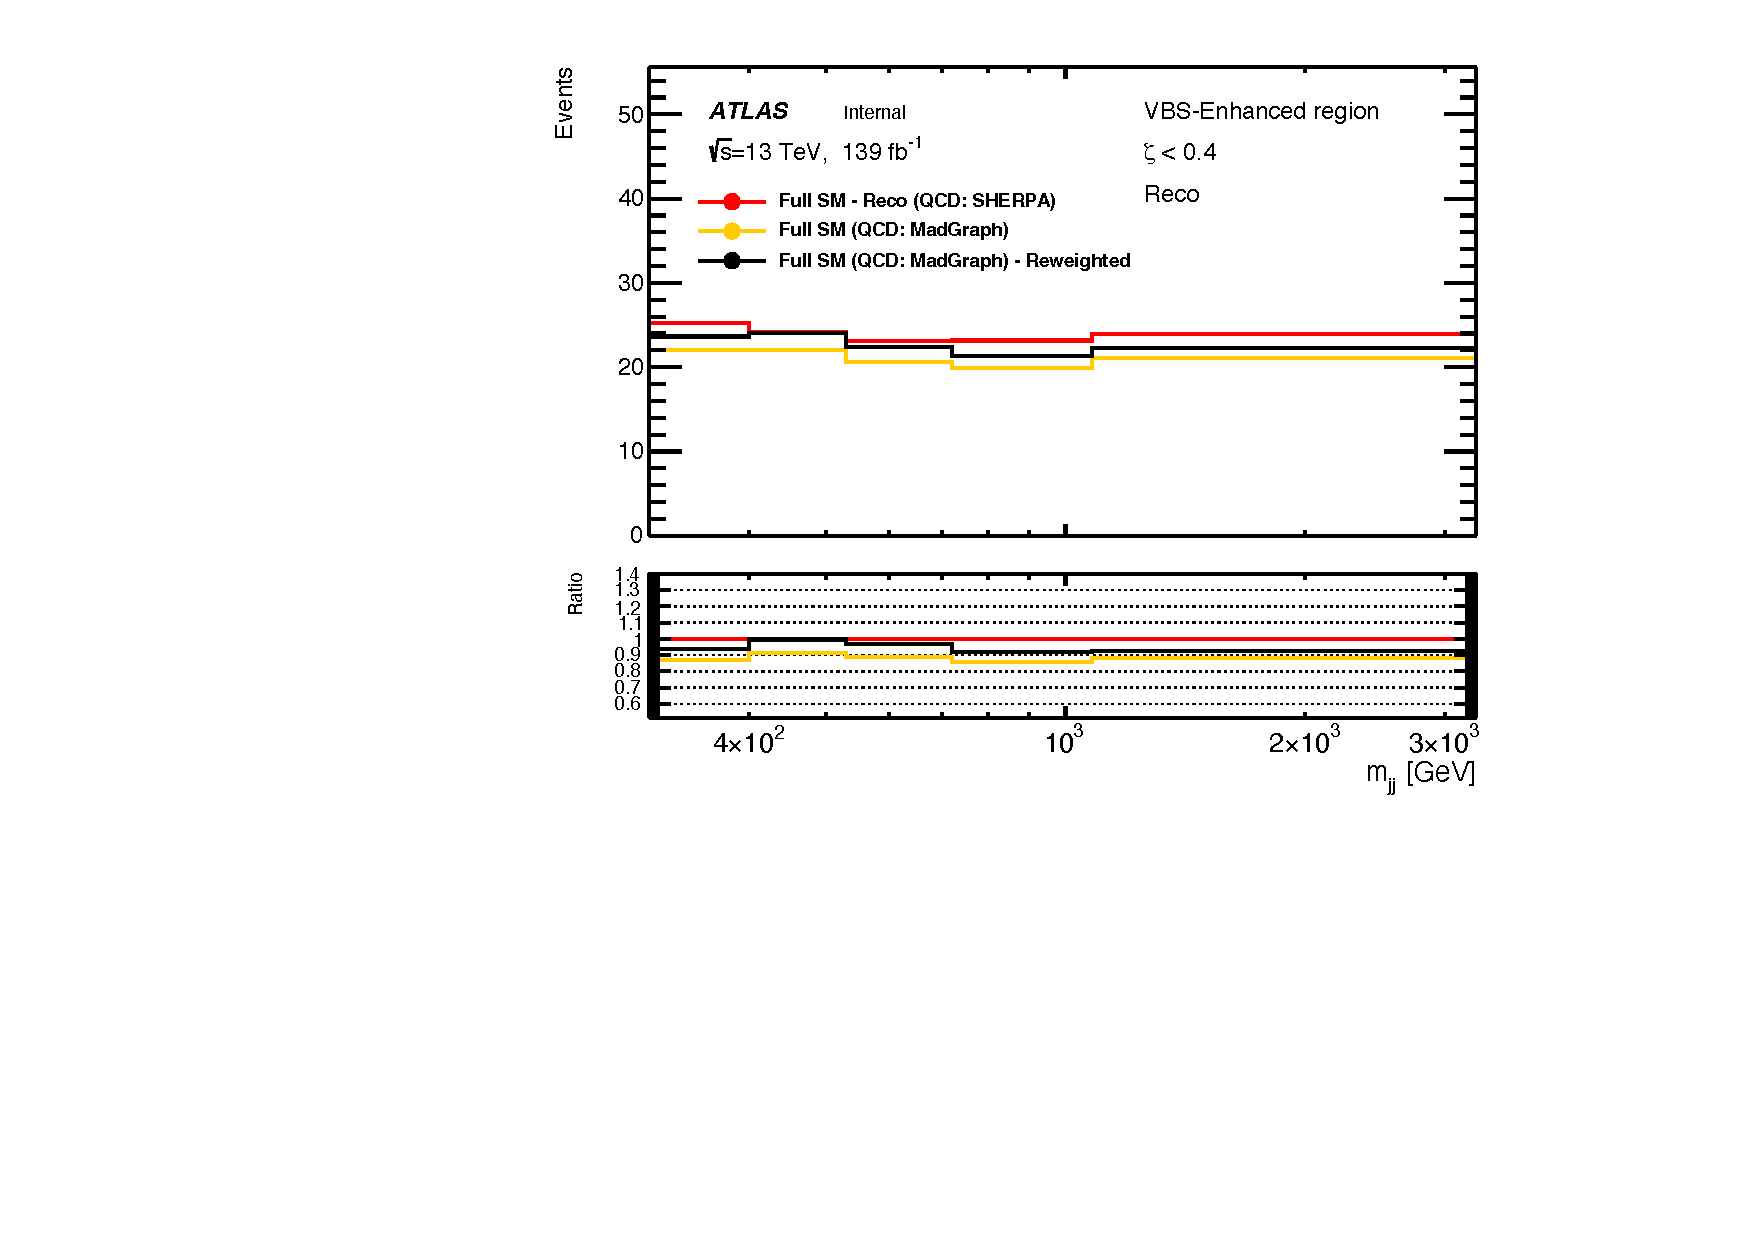
\includegraphics[width=.48\linewidth]{figures/Analysis/Systematics/QCDmodel_Dist.pdf}
        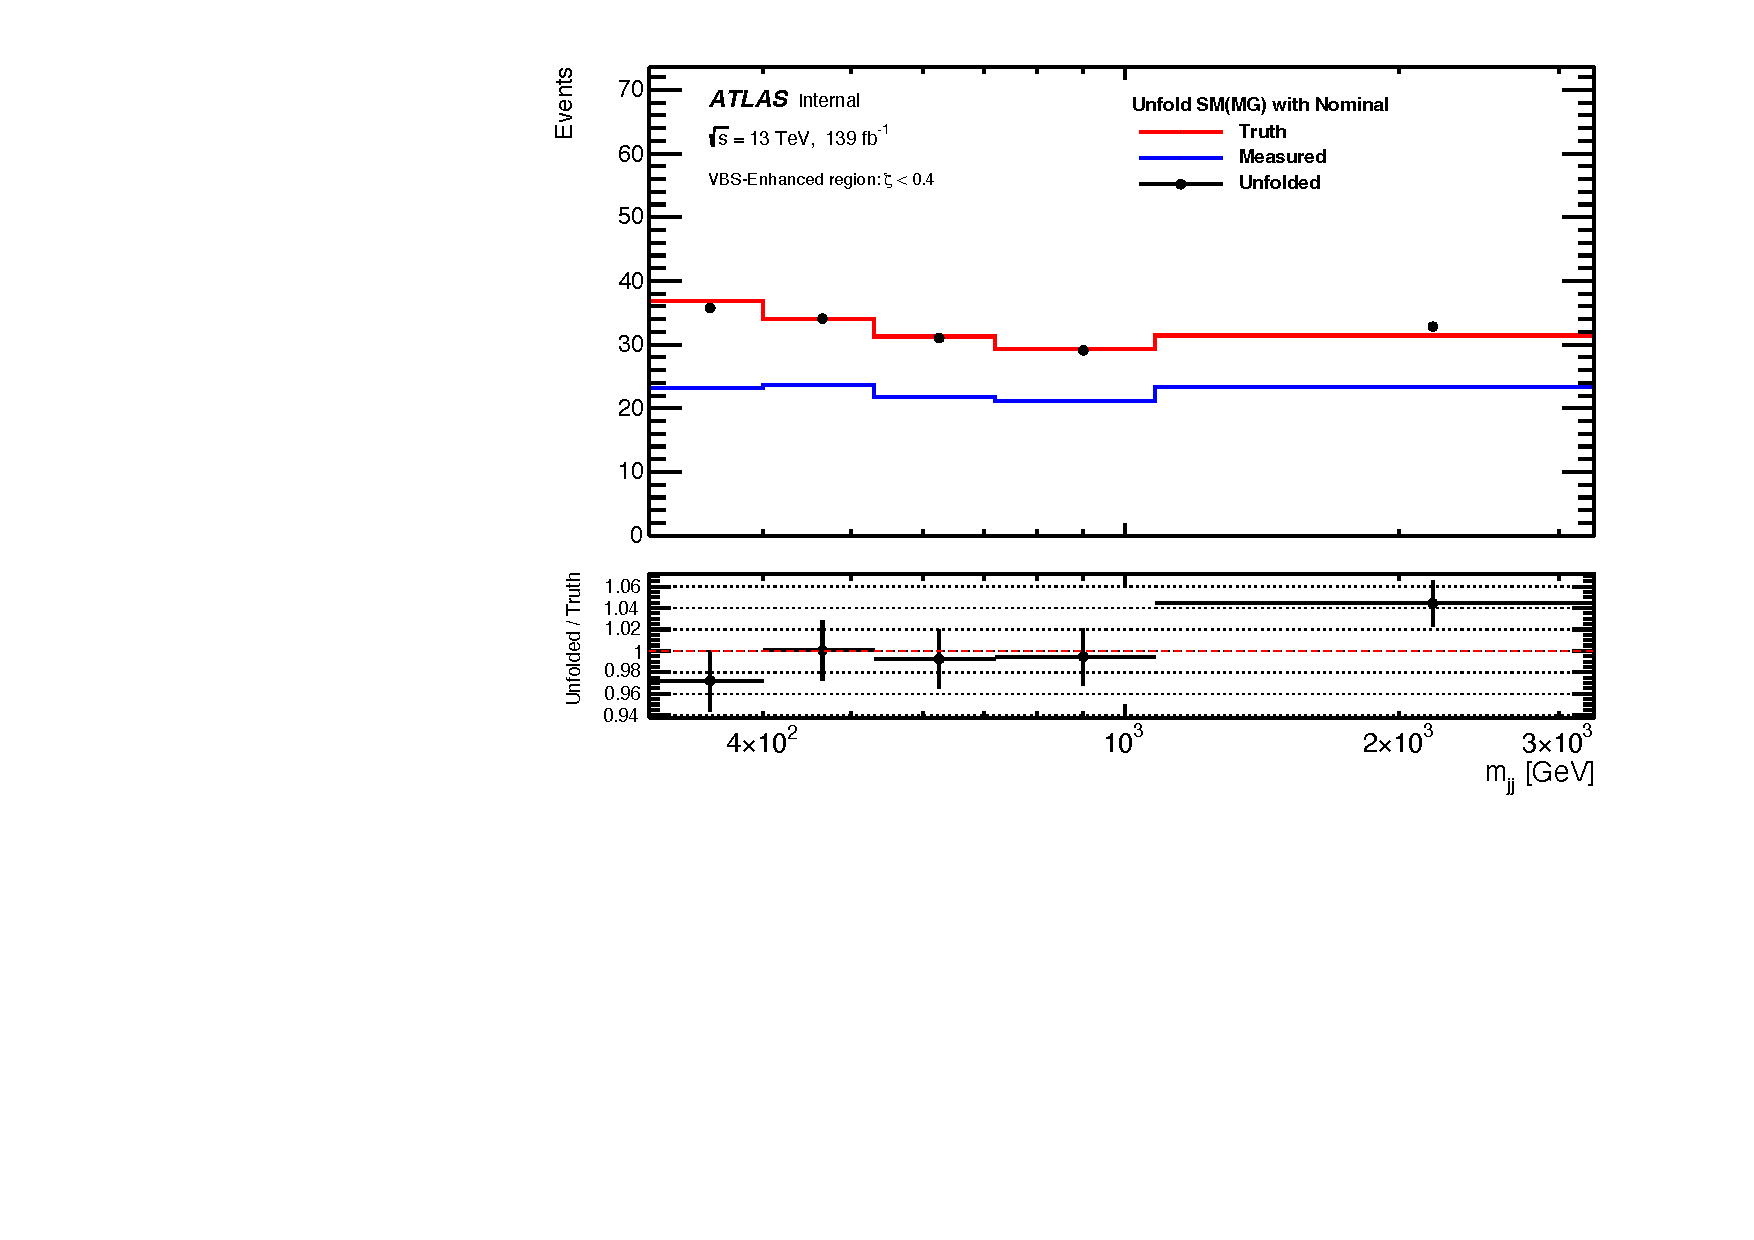
\includegraphics[width=.48\linewidth]{figures/Analysis/Systematics/QCDmodel_Unc.pdf}
        \caption{The left plot shows three distributions of $m_{jj}$ in VBS-Enhanced region at detector-level, red corresponding to SM predictions where $qqZZ$ is taken from \textsc{Sherpa}, yellow shows the same but $qqZZ$ is taken from \textsc{MadGraph5} and black shows the reweighted-\textsc{MadGraph5} distribution to match the \textsc{Sherpa} lineshape. The right plot shows reweighted-\textsc{MadGraph5} detector-level (blue) distribution, which is unfolded (black) using unfolding inputs from nominal-\textsc{Sherpa} and compared to the particle-level reweighted-\textsc{MadGraph5} distribution (red). The ratio panel of the right plot showing the ratio between reweighted truth-level \textsc{MadGraph5} and reweighted unfolded-level \textsc{MadGraph5} gives the QCD modeling uncertainties. \label{fig:QCDModelUnc}}
 \end{figure}  

    }
\end{itemize}

\subsection{Background Uncertainties}
\label{subsec:BkgUnc}
There are additional sources of uncertainties from the data-driven estimate of the fake background. The statistical and systematic uncertainties on the fake efficiency discussed in Section \ref{subsubsec:FakeEff}, estimated in the combined control region, are propagated to the final unfolded cross-section yield. First, the variation-applied fake background is calculated and subtracted from the nominal detector-level prediction for each variation. The subtracted altered distribution is then unfolded with nominal unfolding inputs. The difference between the altered-unfolded distribution and the nominal-unfolded distribution gives the impact of the background uncertainties on the unfolded cross-section measurements.

\subsection{Breakdown of the Systematic Uncertainties }
\label{subsec:SysUncBreakdown}
Tables \ref{tab:systematics_mjj_VBS_Suppressed} and \ref{tab:systematics_mjj_VBS_Enhanced} show the impact of systematic uncertainties in VBS-Suppressed and VBS-Enhanced region respectively for each bin of $m_{jj}$. In both regions and most bins, the unfolding bias is the dominant source of systematic uncertainty, followed by the jet systematics. Figure \ref{fig:systematics_mjj} shows the same systematic uncertainties schematically. Figure \ref{fig:jet_systematics_mjj} shows the impact of different categories of the jet systematic uncertainties. In most bins of $m_{jj}$, the dominant jet uncertainties are from the pile-up energy correction step in the jet calibration. The uncertainties from jet eta-dependent calibration and jet energy resolution are also significant. Overall, the jet reconstruction uncertainties have about $8-9\%$ effect on each bin of the unfolded cross-sections.

\begin{table}
\centering
\begin{tabular}{|l || c | c | c | }
\hline 
Bin $m_{jj}$ [GeV] & [300, 410) & [410, 600) & [600, 1780)\\
\hline 
QCD MC modelling & 1.4 & 0.3 & \textbf{6.6 }\\
Jet & \textbf{7.8} & \textbf{6.6} & \textbf{6.3 }\\
Trigger & 0.32 & 0.07 & 0.081 \\
Leptons & 1.8 & 1.2 & 1.2 \\
PRW & 0.39 & 0.062 & 0.21\\
Theory ($qqZZ$) & 2 & 2.4 & 2.1 \\
Theory (EWK $qqZZjj$) & 0.017 & 0.01 & 0.037 \\
Theory ($ggZZ$) & 0.3 & 0.51 & 0.64 \\
MC Bkg. (ttV+VVV) & 1.6 & 1.7 & 1.6 \\
Fake Bkg. (stat + syst) & 3 & 2.3 & 1.8 \\
Luminosity & 1.7 & 1.7 & 1.7 \\
Data-Driven Closure & \textbf{12} & \textbf{6.3} & \textbf{7.1}\\
\hline
Total & 15 & 10 & 12 \\
\hline
\end{tabular}
\caption{Breakdown of the relative systematic uncertainties ($\%$) for each bin of $\mjj$ in the VBS-Suppressed region. \label{tab:systematics_mjj_VBS_Suppressed}}
\end{table}

\begin{table}
\centering
\begin{tabular}{| l || c | c | c | c | c | }
\hline \hline
Bin $m_{jj}$ [GeV] & [300, 400) & [400, 530) & [530, 720) & [720, 1080) & [1080, 3280)\\
\hline
QCD MC modelling & 2.6 & 0.27 & 0.39 & 1.3 & 3.6\\
Jet & \textbf{7.4} & \textbf{7.6} & \textbf{8.9} & \textbf{8.5} & \textbf{8.9}\\
Trigger & 0.061 & 0.078 & 0.083 & 0.053 & 0.049\\
Leptons & 1.1 & 1.1 & 1.1 & 1.1 & 1.1\\
PRW & 0.38 & 0.58 & 0.79 & 0.83 & 0.59\\
Theory ($qqZZ$) & 2.7 & 2.3 & 2.6 & 1.9 & 0.85\\
Theory (EWK $qqZZjj$) & 0.074 & 0.054 & 0.065 & 0.15 & 0.89\\
Theory ($ggZZ$) & 0.48 & 0.3 & 0.34 & 0.36 & 1.1\\
MC Bkg. (ttV+VVV) & 2.7 & 2.6 & 2.4 & 1.8 & 1.2\\
Fake Bkg. (stat + syst) & 2.4 & 2.5 & 2.5 & 1.7 & 1.5\\
Luminosity & 1.7 & 1.7 & 1.7 & 1.7 & 1.7\\
\hline
Total & 9.3 & 9 & 10 & 9.4 & 10\\
\hline
\end{tabular}
\caption{Breakdown of the relative systematic uncertainties ($\%$) for each bin of $\mjj$ in the VBS-Enhanced region. \textcolor{red}{to update including data-driven closure test. } \label{tab:systematics_mjj_VBS_Enhanced}}
\end{table}

\begin{figure}[!htb]
\centering
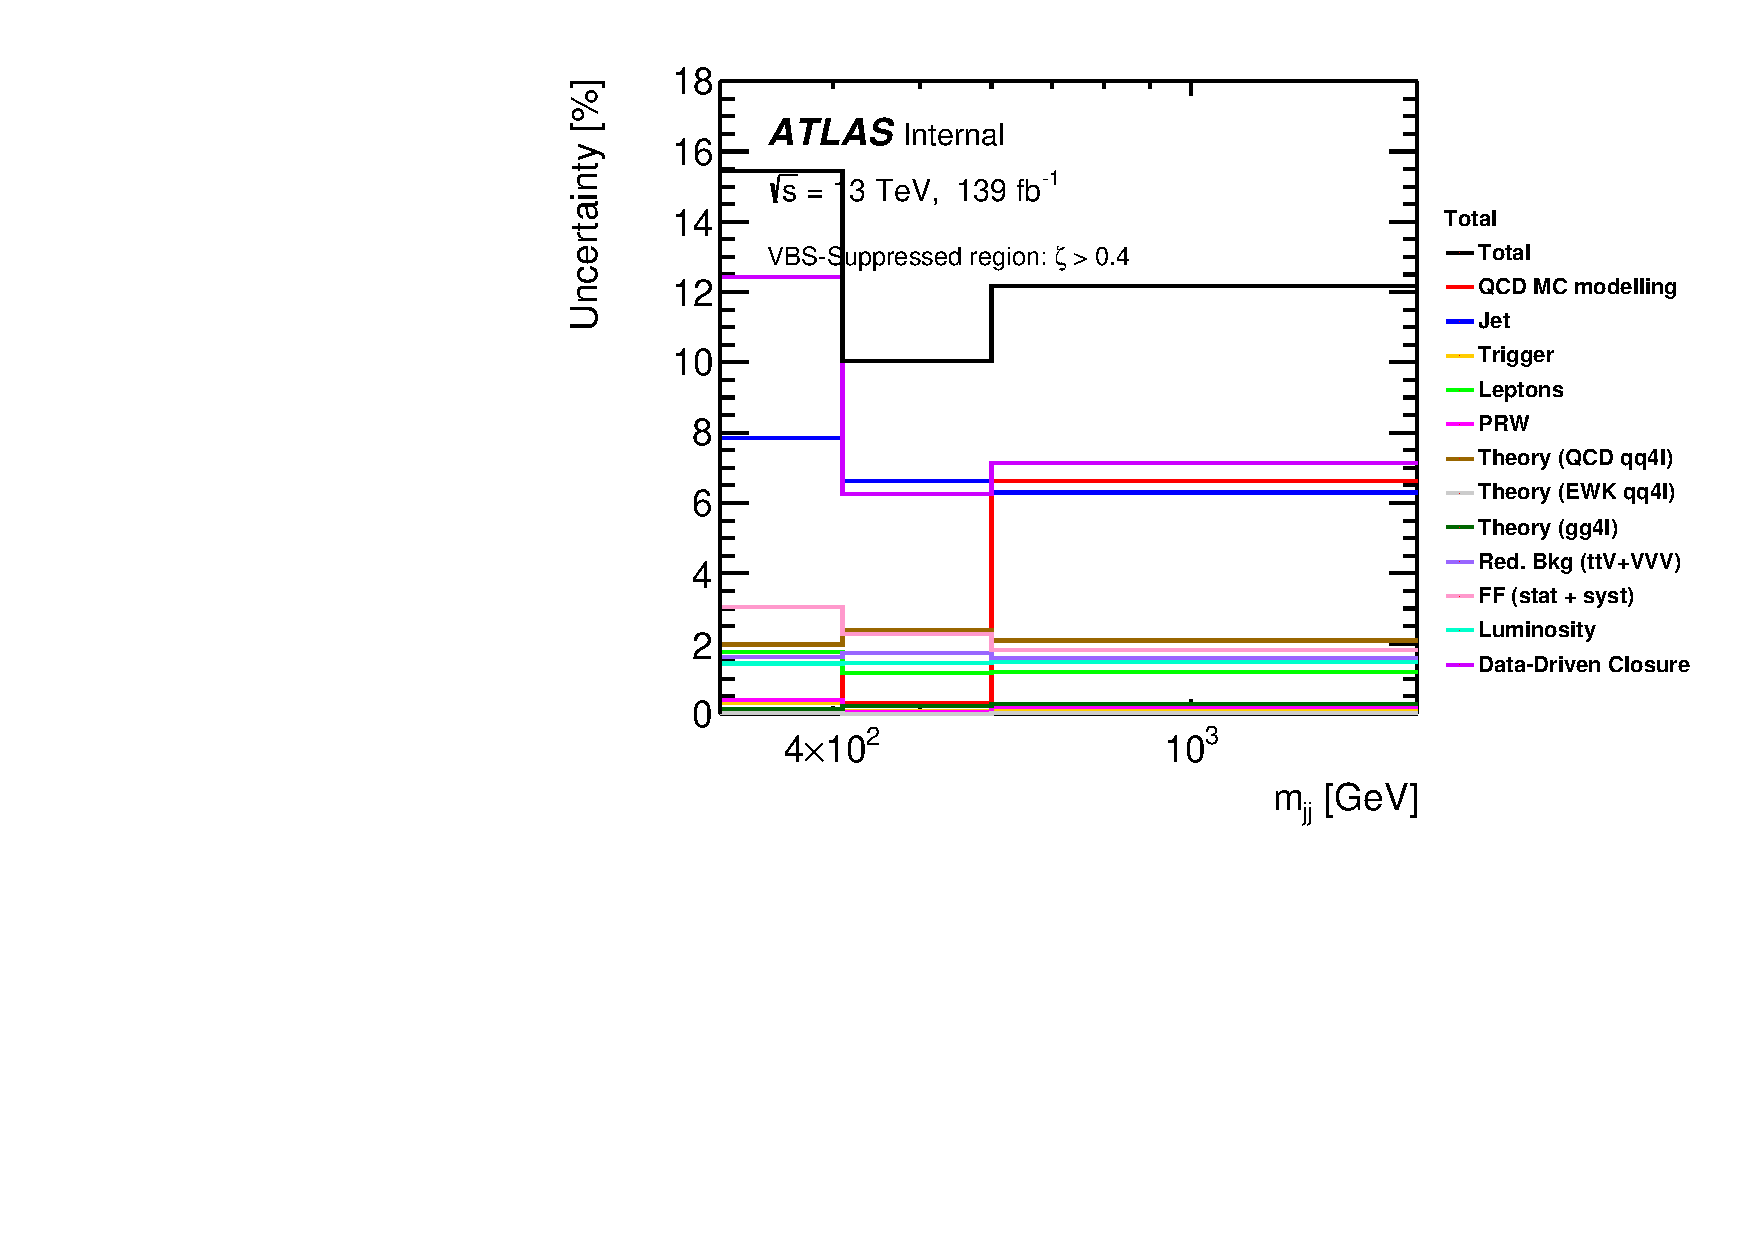
\includegraphics[width=.49\linewidth]{figures/Analysis/Systematics/systematics_VBS_Suppressed.pdf}
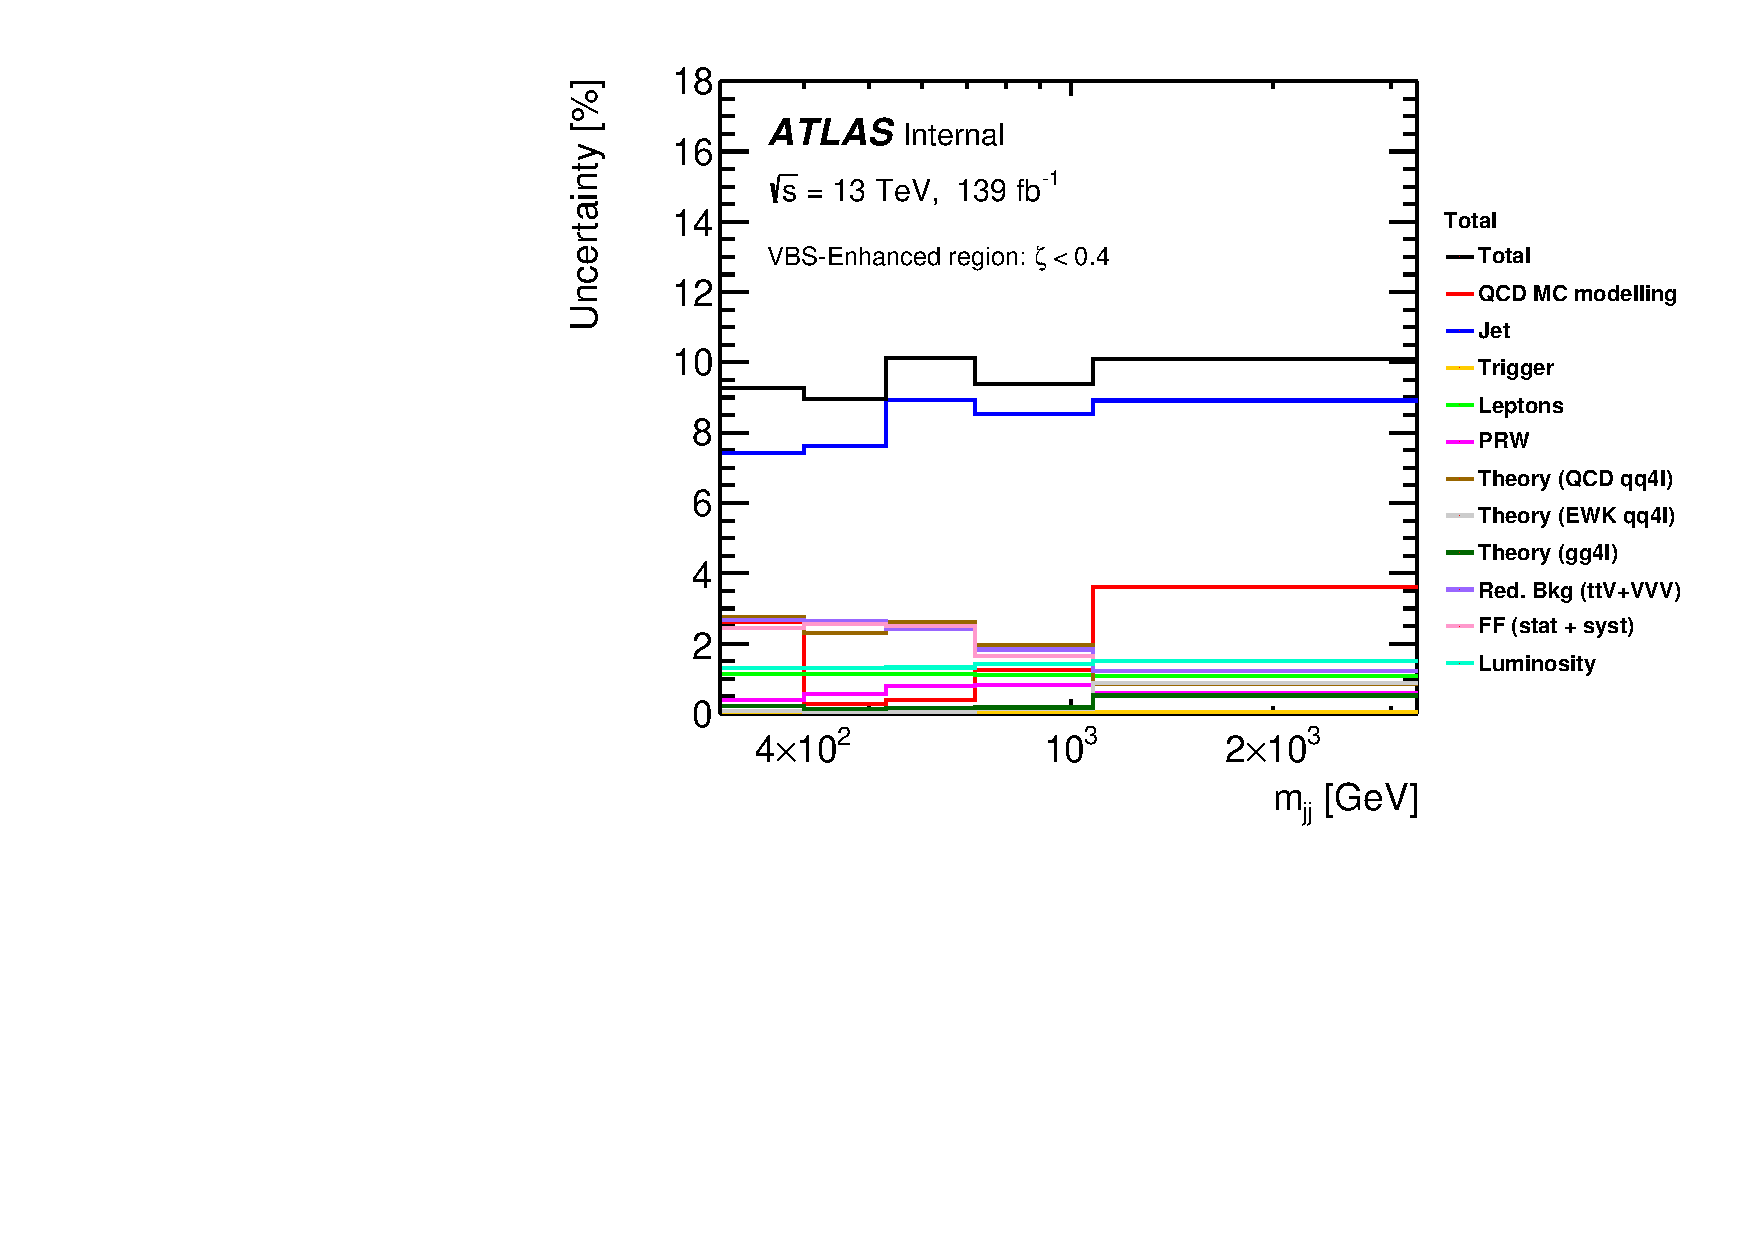
\includegraphics[width=.49\linewidth]{figures/Analysis/Systematics/systematics_VBS_Enhanced.pdf}
\caption{Systematic uncertainties as a function of $\mjj$ in the VBS-Suppressed region (left) and the VBS-Enhanced region (right). \textcolor{red}{update with ATLAS labels and data-driven closure test}}  \label{fig:systematics_mjj}
\end{figure}

\begin{figure}[!htb]
\centering
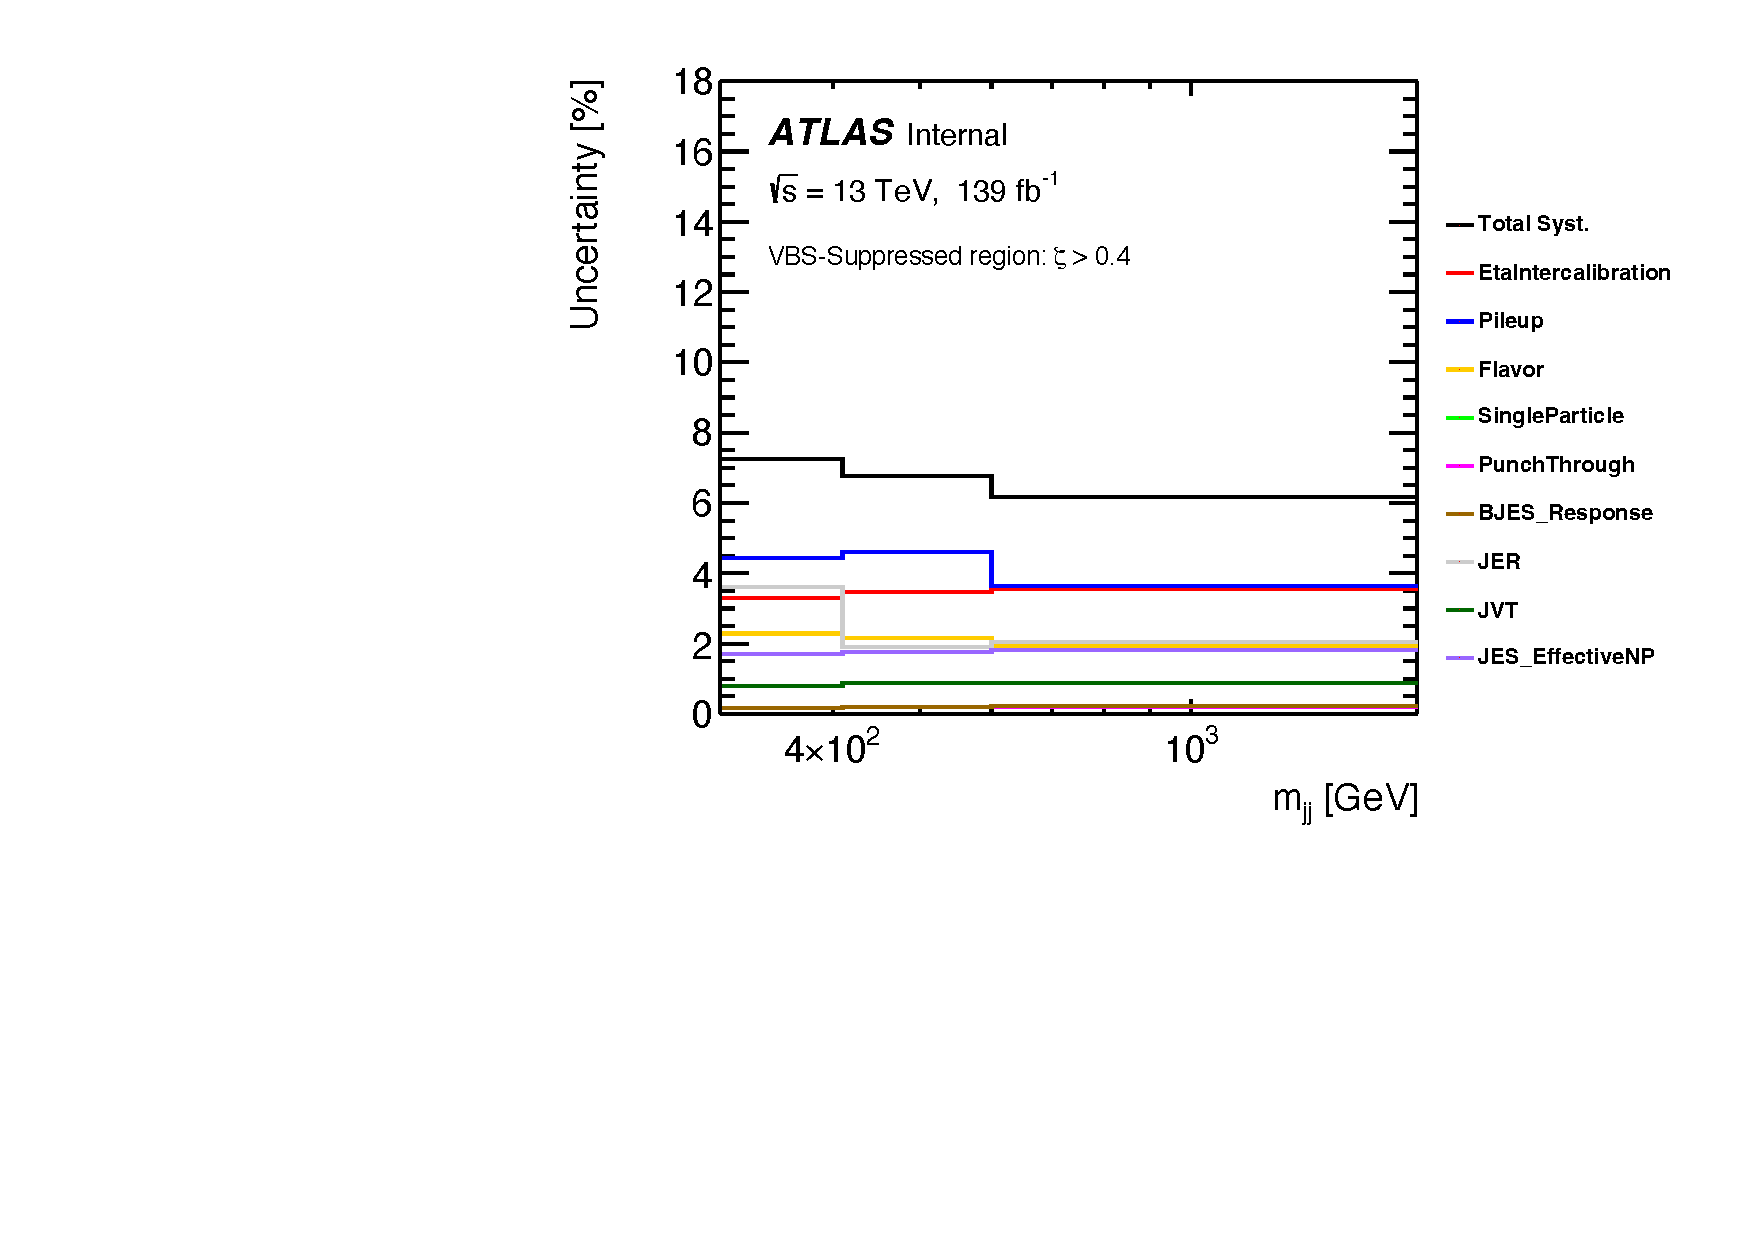
\includegraphics[width=.49\linewidth]{figures/Analysis/Systematics/jet_systematics_VBS_Suppressed.pdf}
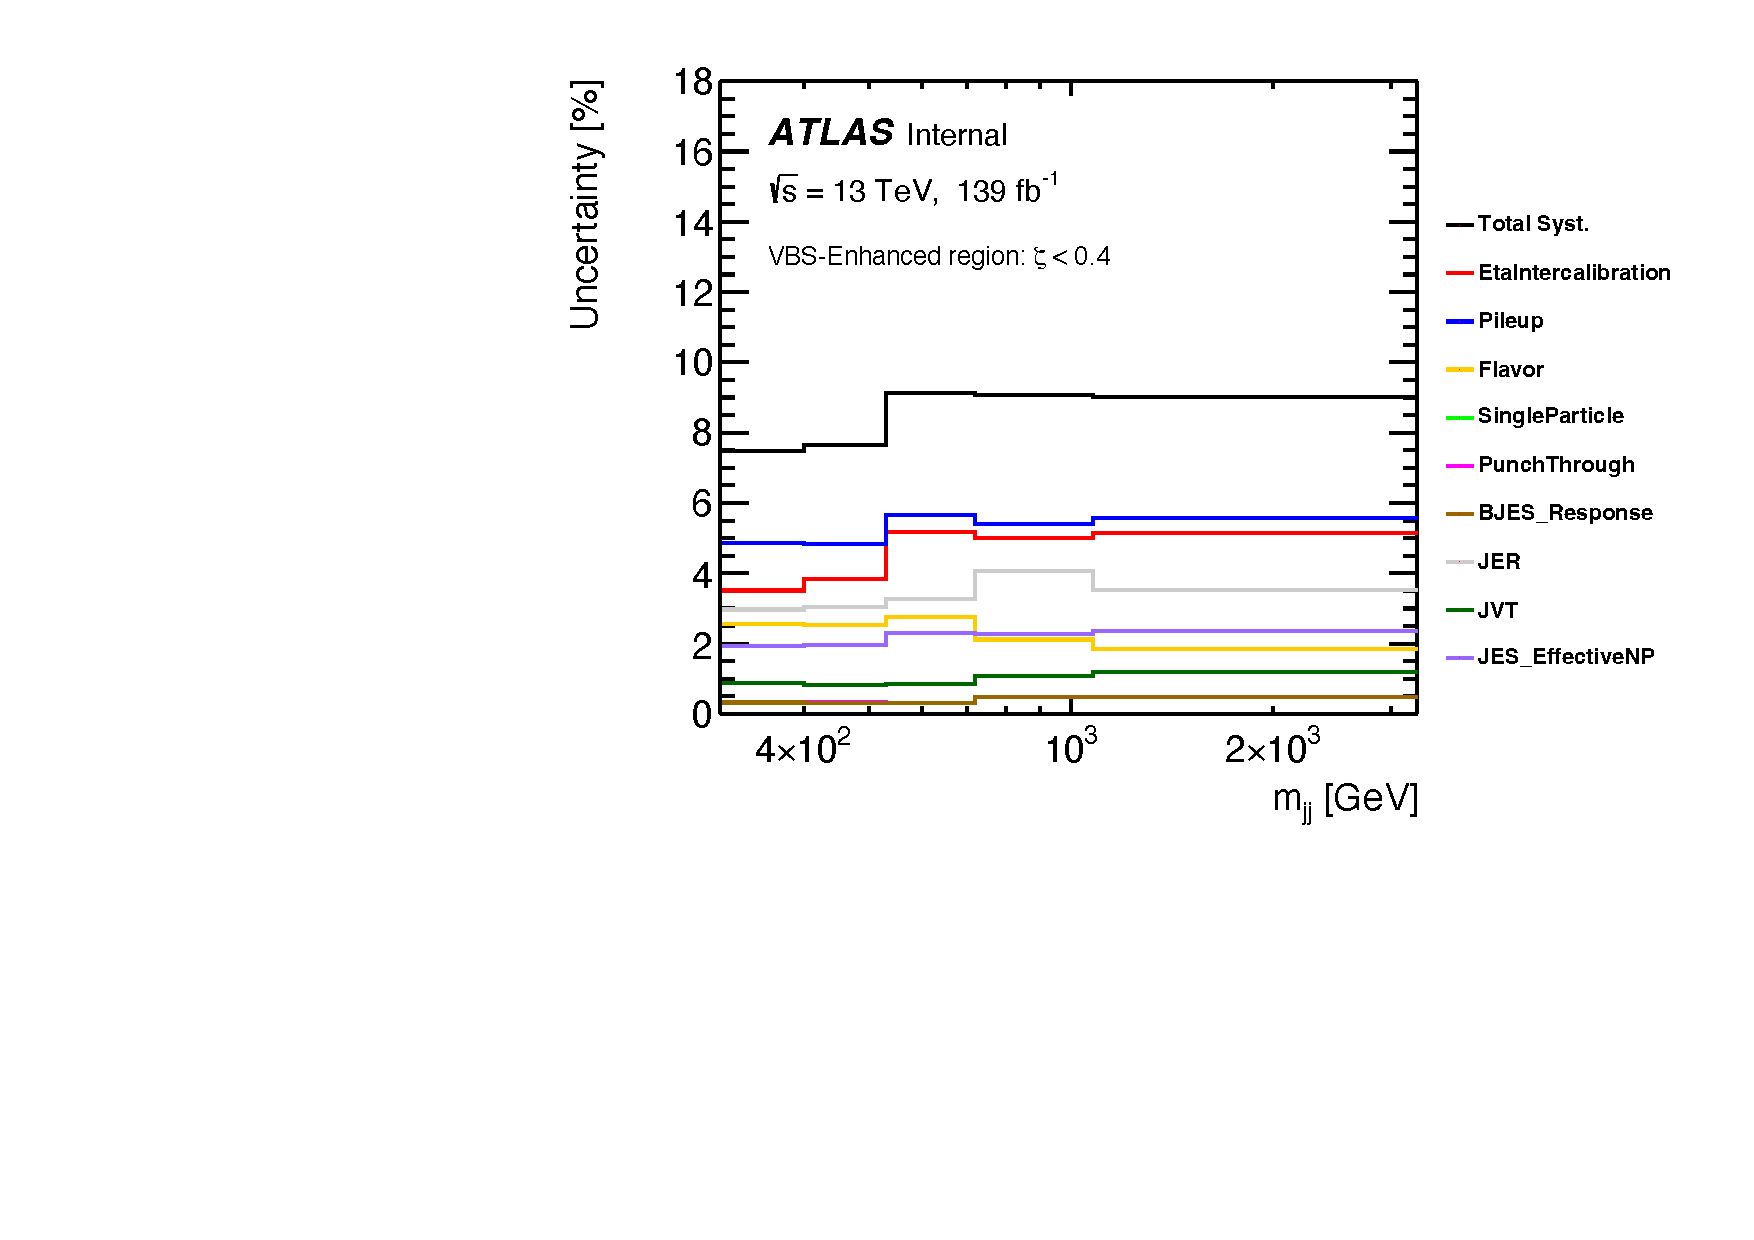
\includegraphics[width=.49\linewidth]{figures/Analysis/Systematics/jet_systematics_VBS_Enhanced.pdf}
\caption{Impact of different jet systematic uncertainties on the unfolded distribution of $\mjj$ in the VBS-Suppressed region (left) and the VBS-Enhanced region (right). \textcolor{red}{update with ATLAS labels and add data-driven closure test}  \label{fig:jet_systematics_mjj}}
\end{figure}

\subsection{Statistical Uncertainties}
\label{subsubsec:StatUnc}
The statistical uncertainty from the reconstructed data needs to be propagated to the estimated unfolded yield. Equation \ref{eqn:BayesianUnfolding} gives the unfolded yield for a target bin i with a single iteration. As the background subtracted detector yields are filled event by event, the reconstruction distribution is uncorrelated. However, as shown by the equation, an unfolded yield in one single bin depends on all detector-level bins due to the resolution effects via bin migration. Therefore, the statistical uncertainty on the unfolded yield is a combination of the uncertainties in detector-level bins and uncertainties on the migration probabilities, which takes the covariance between the detector-level bins into account. The statistical uncertainties at the unfolded level are evaluated by the \textit{RooUnfold} package, which propagates both of these uncertainties.